
\section{Introduction} An auto-encoder is a conceptually simple
neural network used for obtaining useful data representations through
unsupervised training. It is composed of an encoder which outputs a hidden (or
latent) representation and a decoder which attempts to reconstruct the input
using the hidden representation as its input. Training consists of minimizing a
reconstruction cost such as $L_2$ error. However this cost is merely a proxy
for the true objective: to obtain a useful latent representation. Auto-encoders
can  implement many dimensionality reduction techniques such as PCA and Sparse
Coding (SC) ~\cite{DHS}~\cite{SC}~\cite{LISTA}. This makes the study of
auto-encoders very appealing from a theoretical standpoint. In recent years,
renewed interest in auto-encoders networks has mainly been due to their
empirical success in unsupervised feature learning
\cite{SAE1}\cite{SAE2}\cite{CAE}\cite{DAE}. \\

\noindent When minimizing only reconstruction cost, the standard auto-encoder
does not typically learn any meaningful hidden representation of the data. Well
known theoretical and experimental results show that a linear auto-encoder with
trainable encoding and decoding matrices, $W^e$ and $W^d$ respectively, learns
the identity function if $W^e$ and $W^d$ are full rank or over-complete. The
linear auto-encoder learns the principle variance directions (PCA) if $W^e$ and
$W^d$ are rank deficient \cite{DHS}. It has been observed that other
representations can be obtained by regularizing the latent representation. This
approach is exemplified by the Contractive and Sparse Auto-Encoders \cite{CAE}
\cite{SAE1} \cite{SAE2}. Intuitively, an auto-encoder with limited capacity
will focus its resources on reconstructing portions of the input space in which
data samples occur most frequently. From an energy based perspective,
auto-encoders achieve low reconstruction cost in portions of the input space
with high data density (recently, \cite{bengio_new} has examined this
perspective in depth). If the data occupies some low dimensional manifold in
the higher dimensional input space then minimizing reconstruction error
achieves low energy on this manifold. Useful latent state regularizers raise
the energy of points that do not lie on the manifold, thus playing an analogous
role to minimizing the partition function in maximum likelihood models. In this
work we introduce a new type of regularizer that does this explicitly for
auto-encoders with a non-linearity that contains at least one flat (zero
gradient) region. We show examples where this regularizer and the choice of
nonlinearity determine the feature set that is learned by the auto-encoder.      

\section{Latent State Regularization}  Several auto-encoder variants which
regularize their latent states have been proposed, they include the sparse
auto-encoder and the contractive auto-encoder\cite{SAE1}\cite{SAE2}\cite{CAE}.
The sparse auto-encoder includes an over-complete basis in the encoder and
imposes a sparsity inducing (usually $L_1$) penalty on the hidden activations.
This penalty prevents the auto-encoder from learning to reconstruct all
possible points in the input space and focuses the expressive power of the
auto-encoder on representing the data-manifold. Similarly, the contractive
auto-encoder avoids trivial solutions by introducing an auxiliary penalty which
measures the square  Frobenius norm of the Jacobian of the latent
representation with respect to the inputs. This encourages a constant latent
representation except around training samples where it is counteracted by the
reconstruction term. It has been noted in \cite{CAE} that these two approaches
are strongly related. The contractive auto-encoder explicitly encourages small
entries in the Jacobian, whereas the sparse auto-encoder is encouraged to
produce mostly zero (sparse) activations which can be designed to correspond to
mostly flat regions of the nonlinearity, thus also yielding small entries in
the Jacobian.

\subsection{Saturating Auto-Encoder through Complementary Nonlinearities}
Our goal is to introduce a simple new regularizer which explicitly raises
reconstruction error for inputs not near the data manifold. Consider activation
functions with at least one flat region; these include shrink, rectified
linear, and saturated linear (Figure~\ref{fig:nonlin}). Auto-encoders with such
nonlinearities lose their ability to accurately reconstruct inputs which
produce activations in the zero-gradient regions of their activation functions.
Let us denote the auto-encoding function $x_r = G(x,W)$, $x$ being the input,
$W$ the trainable parameters in the auto-encoder, and $x_r$ the reconstruction.
One can define an energy surface through the reconstruction error: \[ E_W(x) =
||x-G(x,W)||^2 \] Let's imagine that $G$ has been trained to produce a low
reconstruction error at a particular data point $x^*$. If $G$ is constant when
$x$ varies along a particular direction $v$, then the energy will grow
quadratically along that particular direction as $x$ moves away from $x^*$. If
$G$ is trained to produce low reconstruction errors on a set of samples while
being subject to a regularizer that tries to make it constant in as many
directions as possible, then the reconstruction energy will act as a {\em
contrast function} that will take low values around areas of high data density
and larger values everywhere else (similarly to a negative log likelihood
function for a density estimator).

The proposed auto-encoder is a simple implementation of this idea.  Using the
notation $W =\{W^e,B^e,W^d,B^d\}$, the auto-encoder function is defined as \[
G(x,W) = W^d F(W^e x+B^e) + B^d \] where $W^e$, $B^e$, $W^d$, and $B^d$ are the
encoding matrix, encoding bias, decoding matrix, and decoding bias,
respectively, and $F$ is the vector function that applies the scalar function
$f$ to each of its components. $f$ will be designed to have "flat spots", i.e.
regions where the derivative is zero (also referred to as the saturation
region).

The loss function minimized by training is the sum of the reconstruction energy
$E_W(x)=||x-G(x,W)||^2$ and a term that pushes the components of $W^e x + B^e$
towards the flat spots of $f$. This is performed through the use of a {\em
complementary function} $f_c$, associated with the non-linearity $f(z)$. The
basic idea is to design $f_c(z)$ so that its value corresponds to the distance
of $z$ to one of the flat spots of $f(z)$. Minimizing $f_c(z)$ will push $z$
towards the flat spots of $f(z)$. With this in mind, we introduce a penalty of
the form $f_c(\sum_{j=1}^d W^e_{ij}x_j + b^e_i)$ which encourages the argument
to be in the saturation regime of the activation function ($f$). We refer to
auto-encoders which include this regularizer as Saturating Auto-Encoders
(SATAEs). For activation functions with zero-gradient regime(s) the
complementary nonlinearity ($f_c$) can be defined as the distance to the
nearest saturation region. Specifically, let $S = \{z \mid  f'(z) = 0\}$ then
we define $f_c(z)$ as: 

\begin{equation} f_c(z) = \inf_ {z' \in S} |z-z'|.   \end{equation}   

\begin{figure} \centering 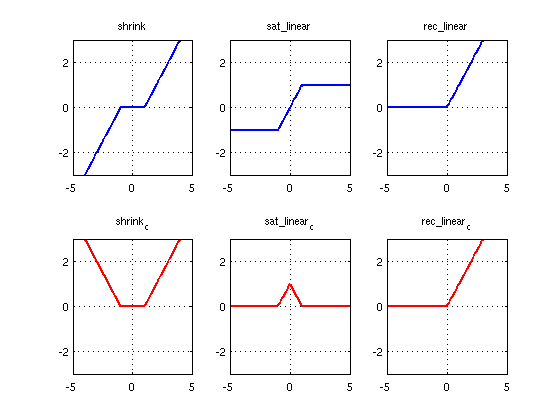
\includegraphics[scale=0.6]{./figures/SATAE/compliments.png}
\caption{Three nonlinearities (top) with their associated complementary
regularization functions(bottom).}  \label{fig:nonlin} \end{figure} 

\noindent Figure 1 shows three activation functions and their associated
complementary nonlinearities. The complete loss to be minimized by a SATAE with
nonlinearity $f$ is: 

\begin{equation} L = \sum_{x \in D} \frac{1}{2} \|x-\left(W^d F(W^e
x+B^e)+B^d\right)\|^2 + \alpha \sum_{i=1}^{d_h}f_c(W^e_i x + b^e_i),
\end{equation}    

\noindent where $d_h$ denotes the number of hidden units. The hyper-parameter
$\alpha$ regulates the trade-off between reconstruction and saturation.  

\section{Effect of the Saturation Regularizer} We will examine the effect of
the saturation regularizer on auto-encoders with a variety of activation
functions. It will be shown that the choice of activation function is a
significant factor in determining the type of basis the SATAE learns. First, we
will present results on toy data in two dimensions followed by results on
higher dimensional image data.

\subsection{Visualizing the Energy Landscape}  Given a trained auto-encoder the
reconstruction error can be evaluated for a given input $x$. For
low-dimensional spaces ($\mathbb{R}^n$, where $n \leq 3$) we can evaluate the
reconstruction error on a regular grid in order to visualize the portions of
the space which are well represented by the auto-encoder. More specifically we
can compute $E(x) = \frac{1}{2} \|x - x_r \|^2$ for all $x$ within some bounded
region of the input space. Ideally, the reconstruction energy will be low for
all $x$ which are in the training set and high elsewhere.
Figures~\ref{fig:toyshrink} and~\ref{fig:toysatlinear} depict the resulting
reconstruction energy for inputs $x \in \mathbb{R}^2$, and  $-1 \leq x_i \leq
1$. Black corresponds to low reconstruction energy. The training data consists
of a one dimensional manifold shown overlain in yellow.
Figure~\ref{fig:toyshrink} shows a toy example for a SATAE which uses ten basis
vectors and a shrink activation function. Note that adding the saturation
regularizer decreases the volume of the space which is well reconstructed,
however good reconstruction is maintained on or near the training data
manifold. The auto-encoder in Figure~\ref{fig:toysatlinear} contains two
encoding basis vectors (red), two decoding basis vectors (green), and uses a
saturated-linear activation function. The encoding and decoding bases are
unconstrained. The unregularized auto-encoder learns an orthogonal basis with a
random orientation. The region of the space which is well reconstructed
corresponds to the outer product of the linear regions of two activation
functions; beyond that the error increases quadratically with the distance.
Including the saturation regularizer induces the auto-encoder basis to align
with the data and to operate in the saturation regime at the extreme points of
the training data, which limits the space which is well reconstructed. Note
that because the encoding and decoding weights are separate and unrestricted,
the encoding weights were scaled up to effectively reduce the width of the
linear regime of the nonlinearity. 

\subsection{SATAE-shrink} Consider a SATAE with a shrink activation function
and shrink parameter $\lambda$. The corresponding complementary nonlinearity,
derived using Equation 1 is given by: \begin{equation} \nonumber shrink_c(x) =
\begin{cases} abs(x), \text{ } |x| > \lambda\\ 0, \text{ elsewhere}
\end{cases}.  \end{equation} 

\begin{figure} \centering 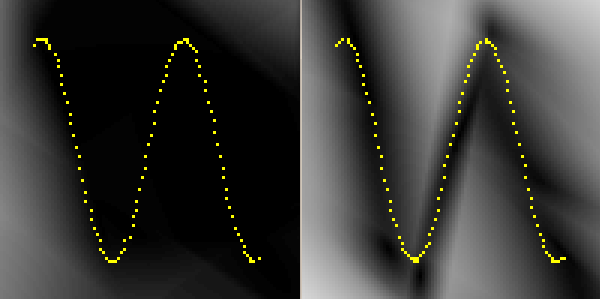
\includegraphics[scale=0.25]{./figures/SATAE/toy_shrink.png}
\caption{Energy surfaces for unregularized (left), and regularized (right)
solutions obtained on SATAE-shrink and 10 basis vectors. Black corresponds to
low reconstruction energy. Training points lie on a one-dimensional manifold
shown in yellow.}  \label{fig:toyshrink} \end{figure} 

\begin{figure} \centering
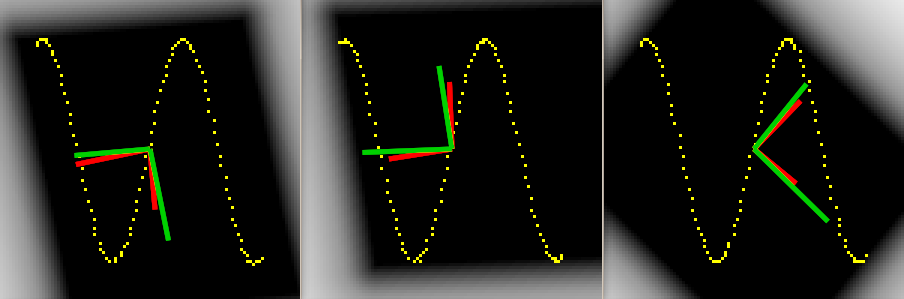
\includegraphics[scale=0.25]{./figures/SATAE/toy_sat_linear_noreg.png}
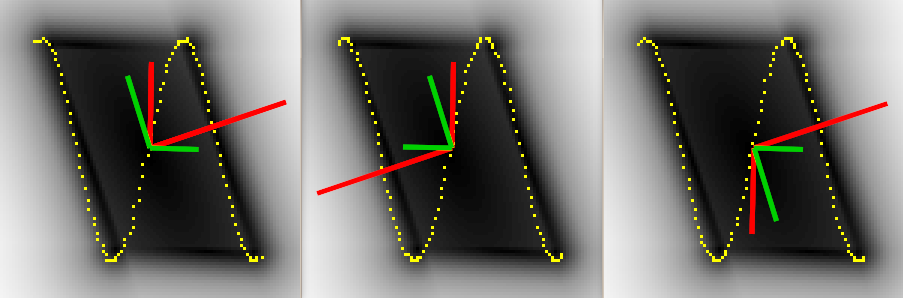
\includegraphics[scale=0.25]{./figures/SATAE/toy_sat_linear_reg.png} \caption{SATAE-SL toy
example with two basis elements. Top Row: three randomly initialized solutions
obtained with no regularization. Bottom Row: three randomly initialized
solutions obtained with regularization.}  \label{fig:toysatlinear} \end{figure} 

Note that $shrink_c(W^e x + b^e) =  abs(shrink(W^e x + b^e))$, which
corresponds to an $L_1$ penalty on the activations. Thus this SATAE is
equivalent to a sparse auto-encoder with a shrink activation function. Given
the equivalence to the sparse auto-encoder we anticipate the same scale
ambiguity which occurs with $L_1$ regularization. This ambiguity can be avoided
by normalizing the decoder weights to unit norm. It is expected that the
SATAE-shrink will learn similar features to those obtained with a sparse
auto-encoder, and indeed this is what we observe. Figure~\ref{fig:results}(c)
shows the decoder filters learned by an auto-encoder with shrink nonlinearity
trained on gray-scale natural image patches. One can recognize the expected
Gabor-like features when the saturation penalty is activated. When trained on
the binary MNIST dataset the learned basis is comprised of portions of digits
and strokes. Nearly identical results are obtained with a SATAE which uses a
rectified-linear activation function. This is because a rectified-linear
function with an encoding bias behaves as a positive only shrink function,
similarly the complementary function is equivalent to a positive only $L_1$
penalty on the activations.          

\afterpage{
\clearpage
\thispagestyle{empty}
\begin{figure} 
\centering \begin{subfigure}[b]{0.225\textwidth} \centering
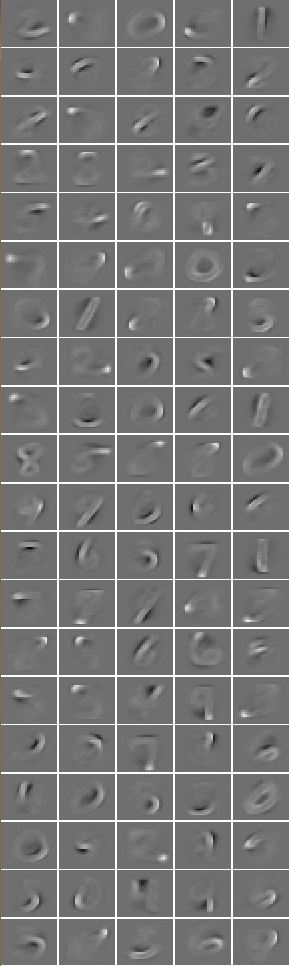
\includegraphics[width=2.5cm, height=10cm]{./figures/SATAE/strokes_full.png} \caption{}
\end{subfigure} \begin{subfigure}[b]{0.225\textwidth} \centering
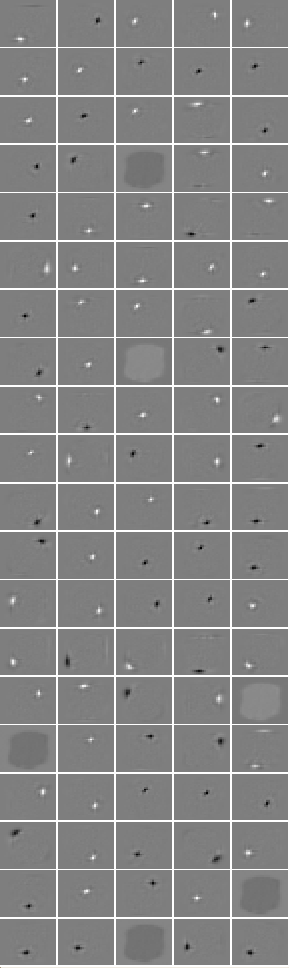
\includegraphics[width=2.5cm, height=10cm]{./figures/SATAE/MNIST_sat_linear_full.png}
\caption{} \end{subfigure} \begin{subfigure}[b]{0.2\textwidth} \centering
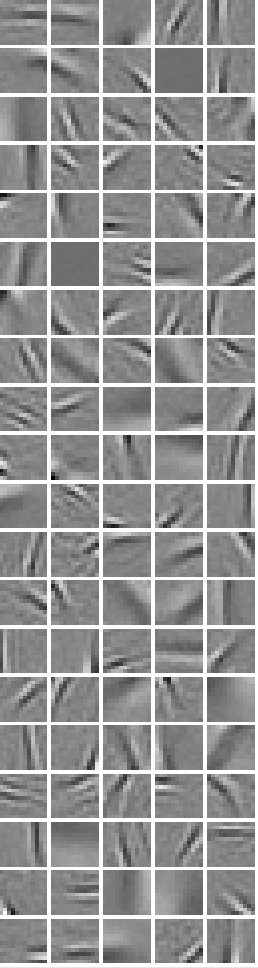
\includegraphics[width=2.5cm, height=10cm]{./figures/SATAE/gabors_full.png} \caption{}
\end{subfigure} \begin{subfigure}[b]{0.2\textwidth} \centering
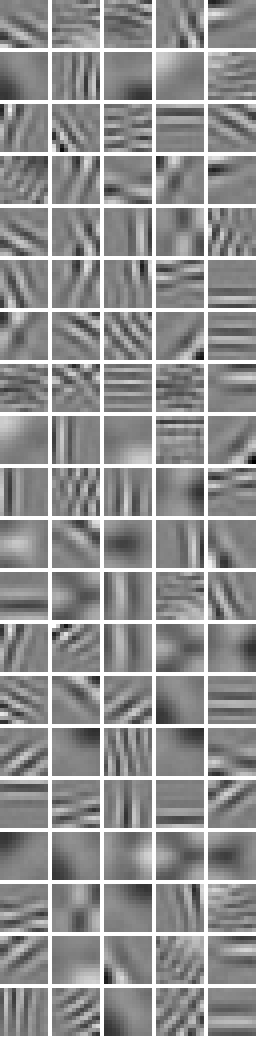
\includegraphics[width=2.5cm, height=10cm]{./figures/SATAE/patches_sat_linear_full.png}
\caption{} \end{subfigure} \\ \begin{subfigure}[b]{0.225\textwidth} \centering
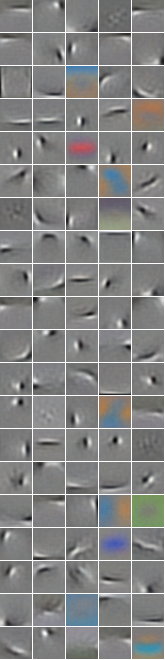
\includegraphics[width=2.5cm, height=10cm]{./figures/SATAE/CIFAR_shrink01.png} \caption{}
\end{subfigure} \begin{subfigure}[b]{0.225\textwidth} \centering
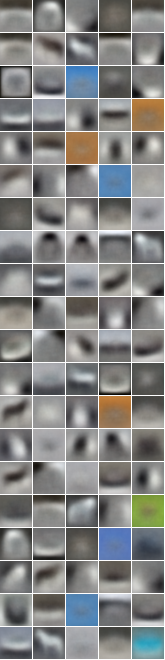
\includegraphics[width=2.5cm, height=10cm]{./figures/SATAE/CIFAR_shrink05.png} \caption{}
\end{subfigure} \begin{subfigure}[b]{0.2\textwidth} \centering
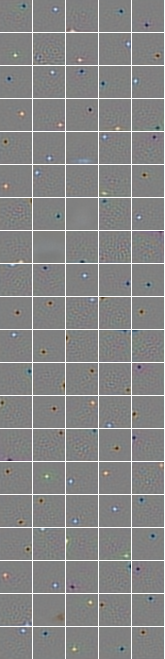
\includegraphics[width=2.5cm, height=10cm]{./figures/SATAE/CIFAR_sat_linear300_1.png}
\caption{} \end{subfigure} \begin{subfigure}[b]{0.2\textwidth} \centering
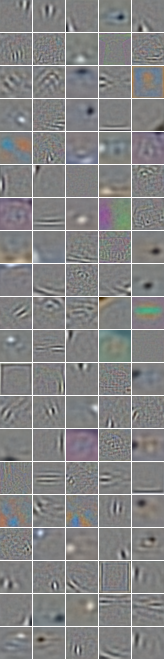
\includegraphics[width=2.5cm, height=10cm]{./figures/SATAE/CIFAR_sat_linear300_6.png}
\caption{} \end{subfigure} \caption{\small Basis elements learned by the SATAE using
different nonlinearities on: 28x28 binary MNIST digits, 12x12 gray scale
natural image patches, and CIFAR-10. (a) SATAE-shrink trained on MNIST, (b)
SATAE-saturated-linear trained on MNIST, (c) SATAE-shrink trained on natural
image patches, (d) SATAE-saturated-linear trained on natural image patches,
(e)-(f) SATAE-shrink trained on CIFAR-10 with $\alpha=0.1$ and $\alpha=0.5$,
respectively, (g)-(h) SATAE-SL trained on CIFAR-10 with $\alpha=0.1$ and
$\alpha=0.6$, respectively.  } \label{fig:results} \end{figure}
\clearpage} 

\begin{figure} \centering 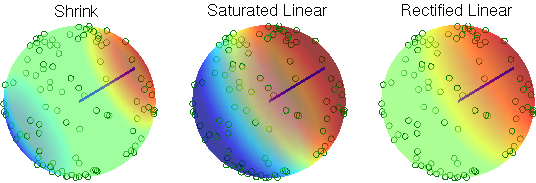
\includegraphics[scale=0.5]{./figures/SATAE/viz_nonlin.png}
\caption{Geometric visualization of non-linearities}
\end{figure} 


\begin{figure} \centering \begin{subfigure}[b]{0.15\textwidth} \centering
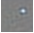
\includegraphics[scale=2]{./figures/SATAE/1.png}\\ 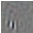
\includegraphics[scale=2]{./figures/SATAE/horse1.png} 
        %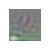
\includegraphics[scale=2]{.//objects/red/0.png} \\
        %\caption{$\alpha=0$}
    \end{subfigure} \begin{subfigure}[b]{0.15\textwidth} \centering
    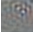
\includegraphics[scale=2]{./figures/SATAE/2.png} \\
    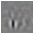
\includegraphics[scale=2]{./figures/SATAE/horse2.png} 
        %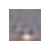
\includegraphics[scale=2]{.//objects/red/1.png} \\
        %\caption{$\alpha=0.1$}
    \end{subfigure} \begin{subfigure}[b]{0.15\textwidth} \centering
    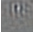
\includegraphics[scale=2]{./figures/SATAE/3.png}\\
    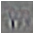
\includegraphics[scale=2]{./figures/SATAE/horse3.png} 
        %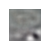
\includegraphics[scale=2]{.//objects/red/2.png} \\
		
        %\caption{$\alpha=0.2$}
    \end{subfigure} \begin{subfigure}[b]{0.15\textwidth} \centering
    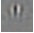
\includegraphics[scale=2]{./figures/SATAE/4.png} \\
    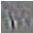
\includegraphics[scale=2]{./figures/SATAE/horse4.png} 
        %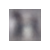
\includegraphics[scale=2]{.//objects/red/3.png} \\
        %\caption{$\alpha=0.5$}
    \end{subfigure} \begin{subfigure}[b]{0.15\textwidth} \centering
    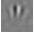
\includegraphics[scale=2]{./figures/SATAE/5.png} 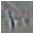
\includegraphics[scale=2]{./figures/SATAE/horse5.png}
    \\
        %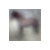
\includegraphics[scale=2]{./objects/red/4.png} \\
		
        %\caption{$\alpha=1$} 
    \end{subfigure} \caption{Evolution of two filters with increasing
    saturation regularization for a SATAE-SL trained on CIFAR-10. Filters
    corresponding to larger values of $\alpha$ were initialized using the
    filter corresponding to the previous $\alpha$. The regularization parameter
    was varied from 0.1 to 0.5 (left to right) in the top five images and 0.5
    to 1 in the bottom five } \label{fig:horse} \end{figure} 

\subsection{SATAE-saturated-linear} Unlike the SATAE-shrink, which tries to
compress the data by minimizing the number of active elements; the SATAE
saturated-linear (SATAE-SL) tries to compress the data by encouraging the
latent code to be as close to binary as possible. Without a saturation penalty
this auto-encoder learns to encode small groups of neighboring pixels. More
precisely, the auto-encoder learns the identity function on all datasets. An
example of such a basis is shown in Figure \ref{fig:results}(b). With this
basis the auto-encoder can perfectly reconstruct any input by producing small
activations which stay within the linear region of the nonlinearity.
Introducing the saturation penalty does not have any effect when training on
binary MNIST. This is because the scaled identity basis is a global minimizer
of Equation 2 for the SATAE-SL on any binary dataset. Such a basis can
perfectly reconstruct any binary input while operating exclusively in the
saturated regions of the activation function, thus incurring no saturation
penalty. On the other hand, introducing the saturation penalty when training on
natural image patches induces the SATAE-SL to learn a more varied basis (Figure
\ref{fig:results}(d)). 

\subsection{Experiments on CIFAR-10} SATAE auto-encoders with 100 and 300 basis
elements were trained on the CIFAR-10 dataset, which contains small color
images of objects from ten categories. In all of our experiments the
auto-encoders were trained by progressively increasing the saturation penalty
(details are provided in the next section). This allowed us to visually track
the effect of the saturation penalty on individual basis elements. Figure
\ref{fig:results}(e)-(f) shows the basis learned by SATAE-shrink with small and
large saturation penalty, respectively. Increasing the saturation penalty has
the expected effect of reducing the number of nonzero activations. As the
saturation penalty increases, active basis elements become responsible for
reconstructing a larger portion of the input. This induces the basis elements
to become less spatially localized. This effect can be seen by comparing
corresponding filters in Figure \ref{fig:results}(e) and (f). Figures
\ref{fig:results}(g)-(h)  show the basis elements learned by SATAE-SL with
small and large saturation penalty, respectively. The basis learned by SATAE-SL
with a small saturation penalty resembles the identity basis, as expected (see
previous subsection). Once the saturation penalty is increased small
activations become more heavily penalized. To increase their activations the
encoding basis elements may increase in magnitude or align themselves with the
input. However, if the encoding and decoding weights are tied (or fixed in
magnitude) then reconstruction error would increase if the weights were merely
scaled up. Thus the basis elements are forced to align with the data in a way
that also facilitates reconstruction. This effect is illustrated in Figure
\ref{fig:horse} where filters corresponding to progressively larger values of
the regularization parameter are shown. The top half of the figure shows how an
element from the identity basis ($\alpha=0.1$) transforms to a localized edge
($\alpha=0.5$). The bottom half of the figure shows how a localized edge
($\alpha=0.5$) progressively transforms to a template of a horse ($\alpha=1$).

\section{Experimental Details} Because the regularizer explicitly encourages
activations in the zero gradient regime of the nonlinearity, many encoder basis
elements would not be updated via back-propagation through the nonlinearity if
the saturation penalty were large. In order to allow the basis elements to
deviate from their initial random states we found it necessary to progressively
increase the saturation penalty. In our experiments the weights obtained at a
minimum of Equation 2 for a smaller value of $\alpha$ were used to initialize
the optimization for a larger value of $\alpha$. Typically, the optimization
began with $\alpha=0$ and was progressively increased to $\alpha=1$ in steps of
$0.1$. The auto-encoder was trained for 30 epochs at each value of $\alpha$.
This approach also allowed us to track the evolution of basis elements as a
function of $\alpha$ (Figure \ref{fig:horse}). In all experiments data samples
were normalized by subtracting the mean and dividing by the standard deviation
of the dataset. The auto-encoders used to obtain the results shown in Figure
\ref{fig:results} (a),(c)-(f) used 100 basis elements, others used 300 basis
elements. Increasing the number of elements in the basis did not have a strong
qualitative effect except to make the features represented by the basis more
localized. The decoder basis elements of the SATAEs with shrink and
rectified-linear nonlinearities were reprojected to the unit sphere after every
10 stochastic gradient updates. The SATAEs which used saturated-linear
activation function were trained with tied weights.  All results presented were
obtained using stochastic gradient descent with a constant learning rate of
0.05.

\section{Discussion}

In this work we have introduced a general and conceptually simple latent state
regularizer. It was demonstrated that a variety of feature sets can be obtained
using a single framework. The utility of these features depend on the
application. In this section we extend the definition of the saturation
regularizer to include functions without a zero-gradient region. The
relationship of SATAEs with other regularized auto-encoders will be discussed.
We conclude with a discussion on future work.   

\subsection{Extension to Differentiable Functions} We would like to extend the
saturation penalty definition (Equation 1) to differentiable functions without
a zero-gradient region. An appealing first guess for the complimentary function
is some positive function of the first derivative, $f_c(x) = |f'(x)|$ for
instance. This may be an appropriate choice for monotonic activation functions
which have their lowest gradient regions at the extrema (e.g. sigmoids).
However some activation functions may contain regions of small or zero gradient
which have negligible extent, at the extrema for instance. We would like our
definition of the complimentary function to not only measure the local gradient
in some region, but to also measure it's extent. For this purpose we employ the
concept of average variation over a finite interval. We define the average
variation of $f$ at $x$ in the positive and negative directions at scale $l$,
respectively as: 

\begin{eqnarray} \nonumber \Delta_l^+ f(x) &=& \frac{1}{l} \int_x ^{x+l}
|f'(u)| du = |f'(x)| * \Pi_l^+(x)\\ \nonumber \Delta_l^- f(x) &=& \frac{1}{l}
\int_{x-l} ^x |f'(u)| du = |f'(x)| * \Pi_l^-(x).  \end{eqnarray} 

Where $*$ denotes the continuous convolution operator. $\Pi_l^+(x)$ and
$\Pi_l^-(x)$ are uniform averaging kernels in the positive and negative
directions, respectively. Next, define a directional measure of variation of
$f$ by integrating the average variation at all scales. 

\begin{eqnarray} \nonumber M^+ f(x) &=& \int_0^{+\infty} \Delta_l^+ f(x) w(l)dl
= \left[\int_0^{+\infty} w(l) \Pi^+_l(x) dl \right] * |f'(x)| \\ \nonumber M^-
f(x) &=& \int_0^{+\infty} \Delta_l^- f(x) w(l)dl = \left[\int_0^{+\infty} w(l)
\Pi^-_l(x) dl \right] * |f'(x)| .  \end{eqnarray} 

Where $w(l)$ is chosen to be a sufficiently fast decreasing function of $l$ to
insure convergence of the integral. The integral with which $|f'(x)|$ is
convolved in the above equation evaluates to some decreasing function of $x$
for $\Pi^+$ with support $x \geq 0$. Similarly, the integral involving $\Pi^-$
evaluates to some increasing function of $x$ with support $x \leq 0$. This
function will depend on $w(l)$. The functions $M^+f(x)$ and $M^-f(x)$ measure
the average variation of $f(x)$ at all scales $l$ in the positive and negative
direction, respectively. We define the complimentary function $f_c(x)$ as: 

\begin{equation} f_c(x) = min(M^+f(x),M^-f(x)).  \end{equation} 

\begin{figure} \centering 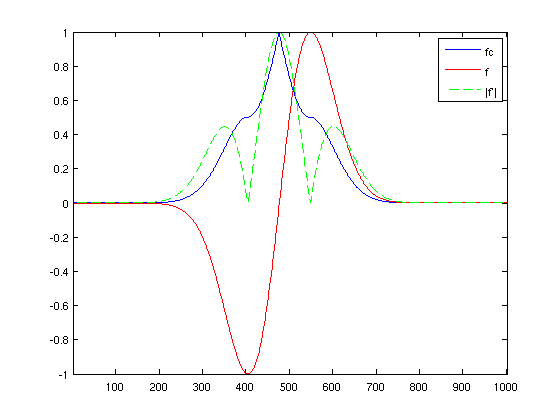
\includegraphics[scale=0.43]{./figures/SATAE/diff_cc.png}
\caption{Illustration of the complimentary function ($f_c$) as defined by
Equation 3 for a non-monotonic activation function ($f$). The absolute
derivative of $f$ is shown for comparison.}  \label{fig:diff_cc} \end{figure} 

An example of a complimentary function defined using the above formulation is
shown in Figure~\ref{fig:diff_cc}. Whereas $|f'(x)|$ is minimized at the
extrema of $f$, the complimentary function only plateaus at these locations.

\subsection{Relationship with the Contractive Auto-Encoder} Let $h_i$ be the
output of the $i^{th}$ hidden unit of a single-layer auto-encoder with
point-wise nonlinearity $f(\cdot)$. The regularizer imposed by the contractive
auto-encoder (CAE) can be expressed as follows: 

\begin{equation} \nonumber \sum_{ij} \left(\frac{\partial h_i}{\partial x_j}
\right)^2 = \sum_i ^{d_h} \left(f'(\sum_{j=1}^d W^e_{ij}x_j + b_i)^2 \| W^e_i
\| ^2 \right), \end{equation}  
 
\noindent where $x$ is a $d$-dimensional data vector, $f'(\cdot)$ is the
derivative of $f(\cdot)$, $b_i$ is the bias of the $i^{th}$ encoding unit, and
$W^e_i$ denotes the $i^{th}$ row of the encoding weight matrix. The first term
in the above equation tries to adjust the weights so as to push the activations
into the low gradient (saturation) regime of the nonlinearity, but is only
defined for differentiable activation functions. Therefore the CAE indirectly
encourages operation in the saturation regime. Computing the Jacobian, however,
can be cumbersome for deep networks. Furthermore, the complexity of computing
the Jacobian is $O(d \times d_h)$, although a more efficient implementation is
possible \cite{CAE}, compared to the $O(d_h)$ for the saturation penalty.  
 
\subsection{Relationship with the Sparse Auto-Encoder} In Section 3.2 it was
shown that SATAEs with shrink or rectified-linear activation functions are
equivalent to a sparse auto-encoder. Interestingly, the fact that the
saturation penalty happens to correspond to $L_1$ regularization in the case of
SATAE-shrink agrees with the findings in \cite{LISTA}. In their efforts to find
an architecture to approximate inference in sparse coding, Gregor et al. found
that the shrink function is particularly compatible with $L_1$ minimization.
Equivalence to sparsity only for some activation functions suggests that SATAEs
are a generalization of sparse auto-encoders. Like the sparsity penalty, the
saturation penalty can be applied at any point in a deep network for the same
computational cost. However, unlike the sparsity penalty the saturation penalty
is adapted to the nonlinearity of the particular layer to which it is applied. 
